\documentclass[12pt]{article}
\usepackage{hyperref}
\usepackage{listings}
\usepackage[margin=1in]{geometry}
\usepackage{enumitem}
\usepackage{multicol}
\usepackage{array}
\usepackage{titlesec}
\usepackage{helvet}
\renewcommand{\familydefault}{\sfdefault}
\usepackage{amsmath}     % For math equations
\usepackage{amssymb}     % For advanced math symbols
\usepackage{amsfonts} % For math fonts
\usepackage{gvv}
\usepackage{esint}
\usepackage[utf8]{inputenc}
\usepackage{graphicx}
\usepackage{pgfplots}
\pgfplotsset{compat=1.18}
\titleformat{\section}{\bfseries\large}{\thesection.}{1em}{}
\setlength{\parindent}{0pt}
\setlength{\parskip}{6pt}
\usepackage{multirow}
\usepackage{float}
\usepackage{caption}


\begin{document}

\section*{Problem 8.3.12}
Find the equation of the set of all points the sum of whose distances 
from the points $\myvec{3\\0}$ and $\myvec{9\\0}$ is $12$.

\section*{Input Variables}
\begin{table}[H]
\centering
\begin{tabular}{|c|c|}
\hline
Variable & Value \\
\hline
$\vec F_1$ & $\myvec{3\\0}$ \\
\hline
$\vec F_2$ & $\myvec{9\\0}$ \\
\hline
$2a$ & $12$ \\
\hline
\end{tabular}
\caption{} \label{}
\end{table}

\section*{Solution}

\subsection*{Step 1: Center and axis data}
\begin{align}
\vec c &= \frac{\vec F_1+\vec F_2}{2}=\myvec{6\\0}, &
\vec v &= \frac{\vec F_2-\vec F_1}{\|\vec F_2-\vec F_1\|}=\myvec{1\\0}, &
c_f &= \frac{\|\vec F_2-\vec F_1\|}{2}=3, &
a &= 6.
\end{align}
Shift to the midpoint frame: $\vec y:=\vec x-\vec c$.

\subsection*{Step 2: Start from the sum-of-distances definition}
\begin{align}
\|\vec y-c_f\vec v\|+\|\vec y+c_f\vec v\|=2a.
\end{align}

\subsection*{Step 3: Eliminate square roots (squaring twice)}
Let $r_\pm:=\|\vec y\pm c_f\vec v\|$. From (2), $r_++r_-=2a$.
\begin{align}
r_+r_- &= 2a^2-\|\vec y\|^2-c_f^2, \\
r_+-r_- &= \frac{2c_f}{a}\,\vec v^\top\vec y
\;\Rightarrow\;
r_+r_- = a^2-\frac{c_f^2}{a^2}(\vec v^\top\vec y)^2.
\end{align}
Equating the two expressions for $r_+r_-$ yields
\begin{align}
\|\vec y\|^2-\frac{c_f^2}{a^2}(\vec v^\top\vec y)^2 = a^2-c_f^2 \;=:\; b^2.
\end{align}

\subsection*{Step 4: Principal directions and the matrix $D$}
Choose an orthonormal basis of principal directions:
\begin{align}
\vec p_1 &= \vec v, \qquad \vec p_2 \perp \vec p_1, \qquad
P:=\myvec{\vec p_1 & \vec p_2} \;\;\text{(orthonormal)}.
\end{align}
Decompose $\vec y$ as $\vec y = \alpha\,\vec p_1 + \beta\,\vec p_2$, where
$\alpha=\vec p_1^\top\vec y=\vec v^\top\vec y$ and $\beta=\vec p_2^\top\vec y$.
Then $\|\vec y\|^2=\alpha^2+\beta^2$. Substituting into (5) gives
\begin{align}
\frac{\alpha^2}{a^2}+\frac{\beta^2}{b^2}=1.
\end{align}
In matrix form this is
\begin{align}
\vec y^\top \Big(P\,\mathrm{diag}\!\big(\tfrac{1}{a^2},\tfrac{1}{b^2}\big)\,P^\top\Big)\vec y = 1.
\end{align}
Hence define
\begin{align}
D := P\,\mathrm{diag}\!\Big(\tfrac{1}{a^2},\tfrac{1}{b^2}\Big)\,P^\top,
\qquad\text{so that}\qquad
(\vec x-\vec c)^\top D\,(\vec x-\vec c)=1. 
\end{align}

\subsection*{Step 5: Specialization to this data}
Here $\vec p_1=\myvec{1\\0},\ \vec p_2=\myvec{0\\1}$, so $P=I$ and
\begin{align}
b^2 &= a^2-c_f^2 = 36-9=27, \\
D &= \mathrm{diag}\!\Big(\tfrac{1}{a^2},\tfrac{1}{b^2}\Big)
= \myvec{\tfrac{1}{36}&0\\[2pt]0&\tfrac{1}{27}}.
\end{align}
Therefore the \textbf{centered matrix equation of the locus} is exactly (9) with
\begin{align}
\boxed{\;(\vec x-\myvec{6\\0})^\top
\myvec{\tfrac{1}{36}&0\\[2pt]0&\tfrac{1}{27}}
(\vec x-\myvec{6\\0})=1\;}
\end{align}

\subsection*{Step 6: General quadratic (matrix) form}
Expanding (9) gives $\vec x^\top V\vec x+2\vec u^\top\vec x+f=0$ with
\begin{align}
V &= D, &
\vec u &= -V\vec c, &
f &= \vec c^\top V\vec c - 1.
\end{align}
Numerically,
\begin{align}
\boxed{\;
V=\myvec{\tfrac{1}{36}&0\\[2pt]0&\tfrac{1}{27}},\quad
\vec u=\myvec{-\tfrac{1}{6}\\[2pt]0},\quad
f=0\; }.
\end{align}

\begin{figure}[H]
    \centering
    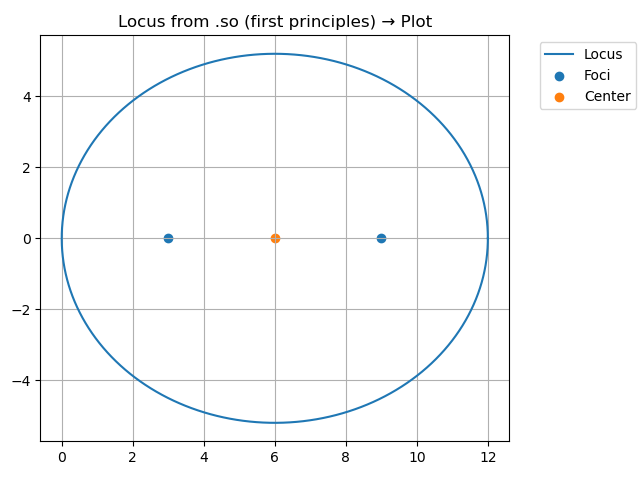
\includegraphics[width=0.9\columnwidth]{figs/ellipse.png}
    \caption{}
    \label{fig:placeholder}
\end{figure}

\end{document}
